% Single-head cross-attention, derived from the supplied architecture description.
% Assumptions: sequence-first matrices; batch axis omitted; linear projections
% are written without bias terms. Decoder and encoder feature widths may differ.
% Compile: pdflatex -no-shell-escape -halt-on-error cross_attention.tex
\documentclass[10pt,tikz,border=9pt]{standalone}
\usepackage[T1]{fontenc}
\usepackage{lmodern,amsmath,amssymb}
\usetikzlibrary{arrows.meta,calc}

\definecolor{ink}{HTML}{14263D}
\definecolor{sourceblue}{HTML}{245A99}
\definecolor{projectionpurple}{HTML}{6B43A6}
\definecolor{attentionteal}{HTML}{087F7B}

\tikzset{
  base/.style={
    rectangle,rounded corners=3pt,line width=.75pt,
    align=center,inner sep=5pt,text=ink
  },
  source/.style={base,draw=sourceblue,fill=sourceblue!5,
    minimum width=26mm,minimum height=14mm},
  projection/.style={base,draw=projectionpurple,fill=projectionpurple!5,
    minimum width=30mm,minimum height=14mm},
  operation/.style={base,draw=attentionteal,fill=attentionteal!5,
    minimum width=32mm,minimum height=14mm},
  flow/.style={-{Latex[length=2.1mm,width=1.5mm]},
    draw=ink!85,line width=.8pt,rounded corners=2pt},
  branch/.style={draw=ink!85,line width=.8pt,rounded corners=2pt},
  note/.style={font=\sffamily\small,text=ink!80,align=center}
}

\begin{document}
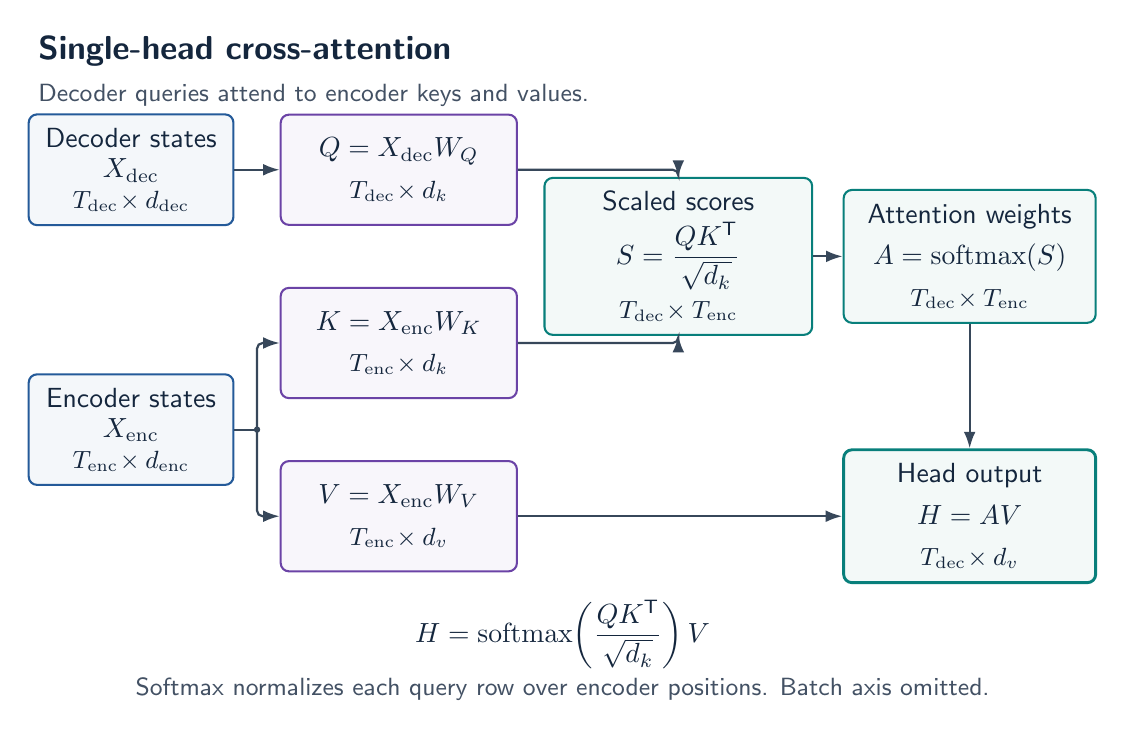
\begin{tikzpicture}[font=\sffamily,text=ink]
  \node[anchor=west,font=\sffamily\large\bfseries] at (-1.3,3.75)
    {Single-head cross-attention};
  \node[anchor=west,note] at (-1.3,3.2)
    {Decoder queries attend to encoder keys and values.};

  % Distinct state sources are essential to cross-attention.
  \node[source] (xdec) at (0,2.25)
    {Decoder states\\[-1pt]$X_{\mathrm{dec}}$\\[-1pt]
     {\small $T_{\mathrm{dec}}\!\times d_{\mathrm{dec}}$}};
  \node[source] (xenc) at (0,-1.05)
    {Encoder states\\[-1pt]$X_{\mathrm{enc}}$\\[-1pt]
     {\small $T_{\mathrm{enc}}\!\times d_{\mathrm{enc}}$}};

  \node[projection] (q) at (3.4,2.25)
    {$Q=X_{\mathrm{dec}}W_Q$\\[3pt]
     {\small $T_{\mathrm{dec}}\!\times d_k$}};
  \node[projection] (k) at (3.4,.05)
    {$K=X_{\mathrm{enc}}W_K$\\[3pt]
     {\small $T_{\mathrm{enc}}\!\times d_k$}};
  \node[projection] (v) at (3.4,-2.15)
    {$V=X_{\mathrm{enc}}W_V$\\[3pt]
     {\small $T_{\mathrm{enc}}\!\times d_v$}};

  \node[operation,minimum width=34mm] (score) at (6.95,1.15)
    {Scaled scores\\[3pt]$S=\dfrac{QK^{\mathsf T}}{\sqrt{d_k}}$\\[3pt]
     {\small $T_{\mathrm{dec}}\!\times T_{\mathrm{enc}}$}};
  \node[operation] (softmax) at (10.65,1.15)
    {Attention weights\\[3pt]$A=\operatorname{softmax}(S)$\\[3pt]
     {\small $T_{\mathrm{dec}}\!\times T_{\mathrm{enc}}$}};
  \node[operation,line width=1.05pt] (out) at (10.65,-2.15)
    {Head output\\[3pt]$H=AV$\\[3pt]
     {\small $T_{\mathrm{dec}}\!\times d_v$}};

  \draw[flow] (xdec.east) -- (q.west);

  % The shared encoder source branches only to keys and values.
  \coordinate (encsplit) at (1.6,-1.05);
  \draw[branch] (xenc.east) -- (encsplit);
  \fill[ink!85] (encsplit) circle[radius=1.15pt];
  \draw[flow] (encsplit) |- (k.west);
  \draw[flow] (encsplit) |- (v.west);

  % Query/key routes enter the two operands of the score calculation.
  \draw[flow] (q.east) -| (score.north);
  \draw[flow] (k.east) -| (score.south);
  \draw[flow] (score.east) -- (softmax.west);
  \draw[flow] (softmax.south) -- (out.north);
  \draw[flow] (v.east) -- (out.west);

  \node[font=\normalsize] at (5.48,-3.65)
    {$\displaystyle H=\operatorname{softmax}\!\left(
      \frac{QK^{\mathsf T}}{\sqrt{d_k}}\right)V$};
  \node[note] at (5.48,-4.35)
    {Softmax normalizes each query row over encoder positions. Batch axis omitted.};
\end{tikzpicture}
\end{document}
